
\documentclass[a4paper,11pt]{article}
% Maths resource packages
\usepackage{amsmath,amssymb,amsfonts,amsthm}
% Packages to allow inclusion of graphics
\usepackage{graphicx}
% For creating hyperlinks in cross references
\usepackage{hyperref}
% Literature reference style
\usepackage[authoryear]{natbib}
\usepackage[bf]{caption}
% Code display
\usepackage[outputdir=build]{minted}
\usepackage{xcolor}
% Import csv-files for tables
\usepackage{csvsimple}


% -----------------------------
% --- user-defined commands ---
% -----------------------------

% insert Quantnet logo
\newcommand{\quantnet}{\raisebox{-1pt}{\includegraphics[scale=0.05]{thesis/figures/qletlogo.pdf}}\,}

% --------------------------
% --- layout definitions ---
% --------------------------

% define topline
\usepackage[automark]{scrpage2}
\pagestyle{scrheadings}
\automark{section}
\clearscrheadings
\ohead{\headmark}

% define citation style
\bibliographystyle{ecta}

% define page size, margin size
\setlength{\headheight}{1.1\baselineskip}
\voffset=-3cm
\hoffset=-3cm
\textheight24cm
\textwidth16cm
\topmargin1cm
\oddsidemargin3cm
\evensidemargin3cm

% define line spacing = 1.5
\renewcommand{\baselinestretch}{1.5}

% define distance between text and footnote line
\addtolength{\skip\footins}{2pc plus 5pt}

% define second level for 'itemizing'
\renewcommand{\labelitemii}{-}

% Minted configuration
\definecolor{friendlybg}{HTML}{f0f0f0}

\setminted[r]{style=friendly, bgcolor=friendlybg,
breaklines, linenos}

\setminted[java]{style=friendly, bgcolor=friendlybg,
breaklines, linenos}



% --------------------------------------
% --------------------------------------
% --------------------------------------
% --- the structure this tex document ---
% frontmatter:
%   - titlepage,
%   - acknowledgement,
%   - abstract,
%   - table of contents,
%   - list of abbreviations,
%   - list of figures,
%   - list of tables.
%
% body of the thesis:
%   - introduction,
%   - methods,
%   - data,
%   - results,
%   - conclusion,
%   - literature,
%   - appendix (figures, tables).
%
% last page:
%   - declaration of authorship.
% --------------------------------------
% --------------------------------------
% --------------------------------------




\begin{document}

% -------------------------------
% --- frontmatter: Title page ---
% -------------------------------

\thispagestyle{empty}
\begin{center}
\vspace{1cm}

    {\Large{\bf Forecasting in blockchain-based smart grids: Solving a prerequisite for the implementation of local energy markets}} \vspace{1cm}


    {\normalsize Master's Thesis submitted\\\vspace{0.5cm}
    to}\\\vspace{0.5cm}
    {\normalsize{\bf Prof. Dr. Wolfgang H\"ardle}} \\\vspace{0.5cm}
    {\normalsize Humboldt-Universit\"at zu Berlin \\
    School of Business and Economics \\
    Ladislaus von Bortkiewicz Chair of Statistics} \vspace{1cm}
    
    \includegraphics[]{thesis/figures/logo.pdf}
    \vspace{1cm}

    {\normalsize by \\\vspace{0.5cm}
    {\bf Michael Kostmann} \\
    (550961)} \vspace{1cm}


    {\normalsize in partial fulfillment of the requirements \\
    for the degree of \\
    {\bf Master of Science} \\
    in Economics and Management Science \\\vspace{1cm}
    Berlin, November 12,  2018}

\end{center}




% ------------------------------------
% --- frontmatter: Acknowledgement ---
% ------------------------------------
\newpage
\pagestyle{plain}
\pagenumbering{roman}   % define page number in roman style
\setcounter{page}{1}    % start page numbering
\section*{Acknowledgement}

I would like to thank Discovergy GmbH for the kind provision of their Smart Meter Data.




% -----------------------------
% --- frontmatter: Abstract ---
% -----------------------------
\newpage
\section*{Abstract}
This document outlines a Master thesis topic. It summaries its relevance, background and related research, describes the data used, proposes methods, and exemplifies the research idea on a small data subsample.
The proposed research aims at implementing prerequisites for the employment of local energy markets on a distributed ledger technology. Such local energy markets have been described and simulated on a Blockchain in previous literature \cite[e.g.,][]{Mengelkamp:2018a}). However, the focus of previous literature has been on the problem of programming such a decentralized market platform in form of a Smart Contract . Fundamental prerequisites for this Smart Contract, such as reliable Smart Meter forecasts of households’ energy consumption and production, have been assumed as given. Thus, how forecasts with a reasonably small error can be computed, is neglected in this literature. This task is particularly challenging under the constraints imposed by the technical implementation of a market mechanism in a Smart Contract on a Blockchain.
Therefore, the proposed study aims to evaluate the possibility of providing such forecasts with existing forecasting methods and realistically available Smart Meter data. An extensive literature review of studies that use high-resolution Smart Meter data to predict individual household energy consumption was conducted. Based on these studies the following forecast-ing techniques seemed most promising and applicable to the task at hand: long short-term memory recurring neural networks (LSTM RNN), pooling-based deep recurring neural net-works (PD RNN), sparse autoregressive LASSO, and distinct wavelet transform (DWT) with Kernel-Wavelet-Functional prediction method (KWF). The best performing prediction technique in terms of four error measures (i.e., MAE, MAPE, NRSME, and MASE) will then be used to assess the effect of forecasting errors on the market mechanism described in \citet{Mengelkamp:2018a}.

%%%%%%%%%%%%%%%%%%%%%%%%%%%%%%%%%%%%%%%%%%%%%%%%%%%%%%%%%%%%%%%%%
This is the template for a thesis at the Chair of Econometrics of
Humboldt--Universit\"at zu Berlin. A popular approach to write a
thesis or a paper is the IMRAD method (Introduction, Methods,
Results and Discussion). This approach is not mandatory! You can
find more information about formal requirements in the booklet
`Hinweise zur Gestaltung der \"au\ss eren Form von Diplomarbeiten' which is available in the office of studies.

The abstract should not be longer than a paragraph of around 10 to 15 lines (or about 150 words). The abstract should contain a
concise description of the econometric/economic problem you
analyse and of your results. This allows the busy reader to obtain quickly a clear idea of the thesis content.




% -----------------------------
% --- frontmatter: Contents ---
% -----------------------------
\newpage
\tableofcontents
\clearpage


% ------------------------------------
% --- frontmatter: List of Figures ---
% ------------------------------------
\newpage
\addcontentsline{toc}{section}{List of Abbreviations}
\ohead[]{LIST OF ABBREVIATIONS}
\section*{List of Abbreviations}

\begin{tabular}{rp{0.2cm}lp{1cm}rp{0.2cm}l}
    LEM     & &  Local energy market    & & XXX     & &  -  \\
    XXX     & &  -                      & & XXX     & &  -
\end{tabular}




% ------------------------------------
% --- frontmatter: List of Figures ---
% ------------------------------------
\newpage
\addcontentsline{toc}{section}{List of Figures}
\ohead[]{\rightmark}
\listoffigures



% -----------------------------------
% --- frontmatter: List of Tables ---
% -----------------------------------
\newpage
\addcontentsline{toc}{section}{List of Tables}
\listoftables



% -------------------------------
% --- main body of the thesis ---
% -------------------------------
\newpage
\pagestyle{plain}
\setcounter{page}{1}    % start page numbering anew
\pagenumbering{arabic}  % page numbers in arabic style



\section{Introduction}\label{Sec:Intro}



%%%%%%%%%%%%%%%%%%%%%%
%%%   Motivation   %%%
%%%%%%%%%%%%%%%%%%%%%%

\subsection{Motivation}\label{Sec:Intro;Subsec:Motivation}

The increasingly wide-spread installation of renewable energy generators currently transforms the German energy landscape substantially \citep{Bayer:2018}. Already in 2016, almost 1.6 million photovoltaic micro-generation units were installed in Germany, according to the Bundesverband Solarwirtschaft \citep{BSW-Solar:2017}. This increasing amount of distributed renewable energy resources combined with a more volatile energy consumption of households –- e.g., due to uncontrolled electric vehicle charging that can increase peak consumption \citep{Fitzgerald:2016,Floch:2017} -– presents a serious challenge for grid operators. As in any electricity grid energy production and consumption always have to be balanced \citep{Weron:2006}, the increasingly volatile and hard to predict energy consumption and production in low voltage grids require new technological solution to manage grid load and energy distribution.

Fortunately, the technological advancement, that lead to the increasing complexity in the energy landscape, also opens up new opportunities to increase the efficiency and reliability of distributed renewable energy production and distribution. As the amount of renewable energy production, that is fed into low voltage grids, has been increasing over the last years \citep{Bayer:2018}, it seems reasonable to shift part of the grid management to lower grid levels. While industry and research already established a comprehensive set of grid management solutions as well as sophisticated consumption and production forecasting techniques for highly aggregated levels, there is still little research on the same topics at lower aggregation levels, such as neighbourhoods or even individual households \citep{Meer:2018}.

One rather recent technological advancement that has the potential to increase the level of energy distribution efficiency on low aggregation level is the implementation of local energy markets on a distributed ledger technology such as blockchain. blockchain has been called an invention similarly revolutionary and paradigm shifting as the Internet \citep{Swan:2015}. While much of the hype around blockchain still has to stand the test against reality, the technology undeniably has the potential to enable new technological solutions. It is not for no reason that more than 20~\% of 70 surveyed German energy executives believe blockchain will be “a game changer for the energy industry” and further 60~\% believe further dispersion of blockchain technology is probable \citep{Burger:2016}. A use case that has been getting special attention due to the media-effective inauguration of the Brooklyn Microgrid \citep{newscientist:2016} is blockchain-based local energy markets.

Local energy markets (LEM) enable localized interconnected energy consumers, producers, and prosumers to trade locally produced energy on a market platform with a specific pricing mechanism \citep{Mengelkamp:2018a}. Major advantages of such local energy markets are (near) real-time pricing and balancing of energy production and consumption in local grids (ibid.). blockchain-based LEM utilise a blockchain as underlying information and communication technology and a smart contract to match supply and demand and settle transactions (ibid.).

However, the product traded on energy markets has some peculiarities compared to other goods. First, energy grids always have to be balanced, i.e. energy demand always has to be matched by energy supply \citep{Weron:2006}. Secondly, as energy is difficult to store, produced energy is fed into the grid mostly instantaneously and continuously and cannot be exchanged in batches of a specific amount at a single point in time. Traditionally, this means that the aggregated energy demand for a geographic area and a specific period of time has to be anticipated and according to this future demand energy is bought and sold. The actual electricity is then produced continuously matching the current demand. This setting is the reasons for today’s existing energy landscape, where utilities and large-scale energy producers and consumers are the only agents involved in electricity markets \citep{Weron:2006}. They trade energy according to the aggregated demand of many consumers. This aggregation makes forecasting future energy demand with relatively small errors \citep{Meer:2018, Wang:2018} and thereby efficient trading possible. Household-level consumers or prosumers, however, do not actively trade but pay their consumption or are reimbursed for their infeed of energy into the grid according to preset tariffs. 

In LEMs, on the contrary, households are the participating market agents. Due to the peculiarities of energy trading mentioned above, the participating households need to forecast their energy demand, respectively supply, to be able to submit a buy or sell offer to the market. This forecasting is substantially harder for single households compared to higher aggregation levels \citep{Wang:2018}.

Therefore, the present research aims to evaluate the possibility of providing such forecasts with existing forecasting methods and realistically available smart meter data with reasonable accuracy. These forecasts are a necessary precondition for LEM and, in particular, the blockchain-based LEM envisioned , e.g., by \citet{Mengelkamp:2018a}.

%%%%%%%%%%%%%%%%%%%%%%%%%%%%
%%%   Related research   %%%
%%%%%%%%%%%%%%%%%%%%%%%%%%%%

\subsection{Related research}\label{Sec:Intro;Subsec:Related}
The present work's topic of concern touches upon three fields of research. The first superordinate topic is local energy markets, their market structure, market mechanism, and market outcomes as well as possible advantages and disadvantages. The second superordinate topic is distributed ledger technology and as such blockchain and smart contracts as well as their use cases for different fields. The third topic is energy forecasting, which encompasses energy consumption forecasting and energy production forecasting. Especially the latter has become increasing attention in the light of increasing adoption of renewable energy resources. All this comes together in blockchain-based local energy markets as implemented in the Brooklyn Microgrid and simulated in the work by \citet{Mengelkamp:2018a}. For such blockchain-based LEM, a necessary prerequisite  is the successful forecast of household-level energy consumption/production based on smart meter recordings. Without this, trading on a market mechanisms as described in \citet{Block:2008} and implemented in a smart contract by \citet{Mengelkamp:2018a} will not possible.


%%%%%%%%%%%
\subsubsection{Local energy markets}
substantial work regarding LEM in general has been done \citep[e.g.,][]{Lamparter:2010, Li:2015, Mihaylov:2014}



%%%%%%%%%%%
\subsubsection{blockchain and smart contracts}



%%%%%%%%%%%
\subsubsection{Local energy markets and blockchain technology}
While substantial work regarding ELM in general has been done (see above), there are only few examples of blockchain-based LEM designs in the existing literature. 
\citet{Mengelkamp:2018b} derive seven principles for microgrid energy markets and evaluate the Brooklyn Microgrid according to those principles. According to the authors knowledge, they are the only ones providing a theoretical framework for the design of blockchain-based LEM and their work may serve as the basis for the future research and implementation of such energy markets.
With a more practical focus, \citet{Mengelkamp:2018a} implemented and simulated a local energy market on a private Ethereum-blockchain  that enables participants to trade local energy production on a decentralized market platform with no need for a central authority.
\citet{Münsing:2017} similarly elaborate a peer-to-peer energy market concept on a blockchain but focus on operational grid constraints and a fair payment rendering. In doing so, they present a decentralized optimal power flow model suitable for implementation on a blockchain.


%%%%%%%%%%%
\subsubsection{Load forecasting of single households}
As mentioned before, the simulations and concepts described in the research above rely on smart meters capable of forecasting the expected energy consumption or production of a household for the next trading interval. This forecasting task is not trivial due to the extremely high volatility of individual private energy consumption \citep{Wang:2018}. Nevertheless, there are several studies trying to forecast different time horizons of smart meter time series.

\citet{Arora:2016} compute probability density estimates for the electricity consumption recorded by individual smart meters in halfhourly intervals from 1000 households and SMEs in Ireland over the course of one year. They employ unconditional and conditional kernel density estimators with a decay parameter to generate point and density forecasts for electricity consumption from 30 minutes to one week ahead.

\citet{Kong:2018} use a long short-term memory deep learning framework to make one time-step ahead forecasts on the AMPds dataset containing half-hourly recordings of energy and appliance usage measurements of a single household in Canada. They show that the prediction accuracy can be improved substantially by including appliance measurement data.

Contrary to this machine learning approach, \citet{Li:2017} use statistical methods to make one time-step ahead forecasts with a sparse autoregressive LASSO model. Using a dataset of 150 consumers from PG\&E with hourly energy consumption recordings for one year, their model captures sparsity in the household’s historical data via LASSO to make a prediction for one household. This prediction is further improved with the historical consumption data of one additional household. This household is identified with the help of a covariance statistic test to identify one other household's data that has the best predictive leverage to improve the original forecast.

On the same dataset as \citet{Arora:2016}, \citet{Shi:2017} use a pooling-based deep recurring neural network to make point forecasts of future consumption and achieve substantial mean absolute percentage error (MAPE) reductions compared to ARIMA, recurring neural network, support vector machine, and deep recurring neural network approaches.

Even though focusing on the forecast of aggregated energy consumption, the work of \citet{Zufferey:2017} shows promising results for forecasting smart meter time series with time delay neural networks (TDNN) using mostly historical features of the time series itself. They use a huge dataset of 40.000 small consumers and 400 photovoltaic power generators in Basel, Switzerland with 15-minute interval recordings of energy consumption and production for one year.

A comprehensive overview on the state of the art of smart meter data analytics is provided by \citet{Wang:2018}. The authors do not only focus on studies researching load forecasting but also provide comprehensive insights into studies regarding smart meter data clustering, preprocessing, load analysis and more. Furthermore, they provide a summary of publicly available smart meter datasets and open research topics.

Notably, there is a lack of standard regarding which forecasting error measures are reported and what benchmark models are used in smart meter data forecasting studies. This is also pointed out by \citet{Meer:2018} in their review paper on probabilistic consumption and production forecasting. Due to this, different forecasting techniques employed in studies using different datasets with partly differing objectives are not directly comparable. 

% Which forecasting techniques should be used in the research proposed here is therefore not directly inferable from the success in applying different forecasting techniques in previous studies.



%%%%%%%%%%%%%%%%%%%%%%%%%%%%
%%%   Present research   %%%
%%%%%%%%%%%%%%%%%%%%%%%%%%%%
\subsection{Present research}\label{Sec:Intro;Subsec:Present}



%%%%%%%%%%%
\subsubsection{Objective}
The aim of the proposed Master thesis is to investigate the prerequisites necessary to implement blockchain-based distributed local energy markets. In particular this is,
\begin{itemize}
    \item[a)] forecasting net energy consumption respectively production of private consumers and prosumers one time-step ahead based only on their historical consumption respectively production data (and potentially calender features),
    \item[b)] evaluate and quantify the effects of forecasting errors, i.e., deviations between forecasted and actual consumption respectively production, for households participating in a LEM, and
    \item[c)] evaluate the implications of variations in forecasting quality for a market mechanism including a settlement mechanism (penalty) for forecasting errors.
\end{itemize}

The underlying setting and technical implementation of the local energy market that is assumed for the present research, is provided by \citet{Mengelkamp:2018a}. The prediction task is fitted to their setup of a local energy market that uses blockchain technology as its information and communication medium and thereby, the present study distinguishes itself notably from previous studies solely trying to forecast smart meter time series in general. Likewise, the evaluation of forecasting errors and their implications is based on their described market mechanism and forecasting error settlement structure and has as such to the authors knowledge not been done in other studies.


%%%%%%%%%%%
\subsubsection{Research questions}
Accordingly, the following research questions are intended to be answered in this study:
\begin{itemize}
    \item[a)] Which prediction technique yields the best 15-minute ahead forecast  for smart meter time series measured in 3-minute intervals using only input features generated from the historical values of the time series and calendar-based features?
    \item[b)] Assuming a forecasting error settlement structure as described in \citet{Mengelkamp:2018a}, what is the quantified loss of households participating in the local energy market due to forecasting errors by the prediction technique identified in a)?
    \item[c)] Depending on the results from b), what implications and potential adjustments for the market mechanism described in \citet{Mengelkamp:2018a} can be identified?
\end{itemize}

The remainder of this thesis is structured as follows: Section~\ref{Sec:Method} presents the forecasting models and the error measures used to evaluate their prediction accuracy. Furthermore, it introduces the market mechanism and the implementation of the market simulation which is used to evaluate the effect of prediction errors on market outcomes. Thereafter, Section~\ref{Sec:Data} describes in detail the data used for this study. As the data has not been used in previous studies, emphasis is put on exposing the characteristics and potential peculiarities of the data at hand. Section~\ref{Sec:Results} presents the prediction results of the forecasting models, evaluates their performance relative to a benchmark model and assesses the effect of prediction errors on market outcomes. The insights gained from this will then be used to identify implications and potential adjustments for future market mechanisms that could be implemented as smart contract in a blockchain. Finally, Section~\ref{Sec:Conc} concludes with a summary, limitations of this study, and an outlook on further research questions emerging from the findings of this thesis.

%%%%%%%%%%%%%%%%%%%%%%%%%%%%%%%%%%%%%%%%%%%%%%%%%%%%%%%%%%%%%%%%%

\section{Method}\label{Sec:Method}



%%%%%%%%%%%%%%%%%%%%%%%%%%%%%%%
%%%   Forecasting methods   %%%
%%%%%%%%%%%%%%%%%%%%%%%%%%%%%%%

\subsection{Forecasting methods}\label{Sec:Method;Subsec:Forecast}



%%%%%%%%%%%
\subsubsection{Benchmark models}



%%%%%%%%%%%
\subsubsection{Long short-term memory recurring neural network}



%%%%%%%%%%%
\subsubsection{Sparse auto-regressive LASSO}



%%%%%%%%%%%%%%%%%%%%%%%%%%
%%%   Error measures   %%%
%%%%%%%%%%%%%%%%%%%%%%%%%%

\subsection{Error measures}\label{Sec:Method;Subsec:Error}



%%%%%%%%%%%
\subsubsection{MAE and RMSE}


%%%%%%%%%%%
\subsubsection{MAPE and NRMSE}



%%%%%%%%%%%
\subsubsection{MASE}



%%%%%%%%%%%
\subsubsection{Ramp score}



%%%%%%%%%%%%%%%%%%%%%%%%%%%%%
%%%   Market simulation   %%%
%%%%%%%%%%%%%%%%%%%%%%%%%%%%%

\subsection{Market simulation}\label{Sec:Method;Subsec:Market}



%%%%%%%%%%%%%%%%%%%%%%%%%%%%%%%%%%%%%%%%%%%%%%%%%%%%%%%%%%%%%%%%%

\begin{itemize}

    \item How was the data analyzed ?

    \item Present the underlying economic model/theory and
        give reasons why it is suitable to answer the given problem.

    \item Present econometric/statistical estimation method and
        give reasons why it is suitable to answer the given problem.

    \item Allows the reader to judge the validity of the study and its findings.

    \item Depending on the topic this section can also be split up into separate sections.

\end{itemize}


\newpage

\section{Data}\label{Sec:Data}



%%%%%%%%%%%%%%%%%%%%%%%
%%%   Data source   %%%
%%%%%%%%%%%%%%%%%%%%%%%

\subsection{Source}\label{Sec:Data;Subsec:Source}

The data used for the present research was provided by Discovergy GmbH.\footnote{The data can be downloaded from \href{https://research.discovergy.com}{https://research.discovergy.com}.} Discovergy installs and maintains smart meters in German households for a one-time installation and monthly maintenance fee. Customers in return get various services centered around the analysis and visualization of their energy consumption and/or production. Discovergy describes itself as a full-range supplier of smart metering solutions offering transparent energy consumption and production data for private and commercial clients \citep{Discovergy:2018}. All energy measurements of their Discovergy smart meters can be accessed by customers through a web portal and mobile app. Additionally, various services are offered, such as, tips for energy savings potential, irregular consumption pattern warnings, personal energy reporting, and consumption analysis of individual appliances.

To be able to offer such data-driven services, Discovergy smart meters\footnote{Discovergy currently installs for private household clients the EasyMeter Q3D standard load profile meter which is connected to the Discovergy Meteorit TM smart meter gateway which records and transmits the recordings to Discovergy servers. The meter specifications can be found here: \texttt{https://discovergy.com/files/sources/product-information/SLP\_Zaehler.pdf} (in German).} record energy consumption and production near real-time -- i.e., 2-second intervals –- and send the readings to Discovergy's servers for storage and analysis. Therefore, Discovergy has extremely high resolution energy data of their customers at their disposal. This high resolution is in stark contrast to the half-hourly or even hourly recorded data used in previous studies \cite[e.g.,][]{Arora:2016,Auder:2018,Shi:2017,Gerossier:2017}.

To the authors knowledge, there is no research using Discovergy smart meter data, apart from \cite{Teixeira:2017} who used the data as simulation input but not for analysis or prediction. As Discovergy never provided data for external research purposes before, there was no suitable process to retrieve data from their internal data storage solutions available. For this reason, the author had to provide an API client for the Discovergy REST API to export data from pre-selected meters.


%%%%%%%%%%%%%%%%%%%%%%
%%%   Obtainment   %%%
%%%%%%%%%%%%%%%%%%%%%%

\subsection{Obtainment}\label{Sec:Data;Subsec:Obtainment}

As all Discovergy smart meters send their measurements in real-time to servers for storage, visualization and analysis, customers can access their meters and measurements through a web application and app. Additionally, customers with the need for automated data access can interact with the stored meter measurements through predefined endpoints. These endpoints serve as an application programming interface (API) called Discovergy REST API \citep{DiscovergyAPI:2018}. By providing the credentials for their Discovergy account\footnote{Sign up for a Discovergy account is open to everyone at https://my.discovergy.com/login. The account provides access to the Discovergy API for developers, without the need of being a Discovergy customer. However, only customers with an installed Discovergy smart meter, that is associated with their account, will have access to actual smart meter data. For testing purposes though, the Discovergy customer service can associate dummy meters as the one used for the demo web portal (\href{https://my.discovergy.com/dashboard?1}{https://my.discovergy.com/dashboard?1}) with any account.}, developers can send requests to a specified endpoint URL. The API returns to such a request a data object formatted in JavaScript Object Notation (JSON). For example, a user authenticates herself with her account credentials and requests the endpoint \texttt{/meters} with the verb \texttt{GET} at the base URL \texttt{https://api.discovergy.com/public/v1}. In response, the server returns a JSON object containing all meter IDs the user has access to.

To automate the process of data retrieval from the Discovergy servers, the author of this study had to program an API client, which is compliant with the constraints of a RESTful architecture.\footnote{REST refers to Representational State Transfer and describes an architetural style that ensures interoperability of systems through the web \cite[][Ch. 5]{fielding:2000}.} This client  had to be able to authenticate the user with account credentials provided in a flat file, request the readings for one year in 3-minute intervals of all meters specified in another flat file, and export the returned JSON data to a specified path. As the API had restrictions on the maximum time span of readings that could be returned depending on the measurement resolution (i.e., returns at most 10 days in 3-minute resolution), the client had to to make 37 request per meter to cover the whole year of 2017 in 10 day periods. As mentioned above, the measurement resolution of the Discovergy smart meters is with 2-second intervals much higher than the 3-minute intervals requested. However, the data management system employed by Discovergy already provides 3-minute aggregations of the original recordings which can be retrieved by specifying the according parameter in the API client.

The client was developed in Java based on the demo client provided in the Discovergy REST API documentation \citep{DiscovergyAPI:2018}. The code for the API client can be found in Appendix \ref{App:Code:C1API}. The client was sent to an Discovergy employee who used an administrative account with access to a sufficiently large number of smart meters to retrieve the data sets used in this study. Unfortunately, it is not known to the author what selection criteria, other than having complete data for all of 2017, where used by Discovergy internally to chose the meters of which the data was provided. Therefore, it is not possible to evaluate how representative the provided data is regarding Discovergy customers or even energy consuming/producing household in general.
After retrieving the data, Discovergy converted the data to csv-files. To facilitate the file transfer, the resulting files were made available online and can by now be downloaded by the general public here: \href{https://research.discovergy.com}{https://research.discovergy.com}. 



%%%%%%%%%%%%%%%%%%%%%%%%%%%%
%%%   Data description   %%%
%%%%%%%%%%%%%%%%%%%%%%%%%%%%

\subsection{Description}\label{Sec:Data;Subsec:Description}

The data comes in 200 individual csv-files each containing the meter readings of a single smart meter. The readings are recorded in 3-minute intervals and range from 01.01.2017 00:00:00 to 01.01.2018 00:00:00. This translates into 175,201 observations per smart meter. Each smart meter measures energy consumption,  energy production and power over all phases installed in the meter and records them together with a timestamp in Unix milliseconds. For this research, only energy consumption and production are relevant. In summary, the data used here are 200 individual data sets each containing two time series (energy consumption and energy production) with 175,201 observations evenly spaced in 3-minute intervals.

Below, a preprocessed and correctly formatted sample of the data for consumer 56 and prosumer 89 containing 6 measurement points are shown.

\begin{table}[ht]
    \csvreader[centered tabular=c|cc,
    table head=
    \hline\hline
    \textbf{time} & \textbf{energy} & \textbf{energyOut} \\
    \hline
    \ldots & \ldots & \ldots \\,
    head to column names,
    separator=comma,
    respect all,
    late after line=\\,
    table foot=
    \ldots &  \ldots & \ldots \\\hline\hline]
    {tables/consumer-00000056_glimpse.csv}{}%
    {\csvcolii & \csvcoliii & \csvcoliv}%
    \caption[Data excerpt of consumer 056]{Data excerpt of consumer 056. \quantnet}
\end{table}

\begin{table}[ht]
    \csvreader[centered tabular=c|cc,
    table head=
    \hline\hline
    \textbf{time} & \textbf{energy} & \textbf{energyOut} \\
    \hline
    \ldots & \ldots & \ldots \\,
    head to column names,
    separator = comma,
    respect all,
    late after line = \\,
    table foot = \ldots & \ldots & \ldots \\\hline\hline]
    {tables/producer-00000089_glimpse.csv}{}%
    {\csvcolii & \csvcoliii & \csvcoliv}%
    \caption[Data excerpt of prosumer 089]{Data excerpt of consumer 089. \quantnet}
\end{table}

The energy and energy out measurements are recorded in the unit $10^{-10}$ kWh. \texttt{energy} records the meter's energy consumption reading at time $t$ (i.e., for example, up until 2017-09-20 12:18:00, consumer 056 consumed \csvreader[
filter equal = {\thecsvinputline}{2}]%
{tables/consumer-00000056_glimpse.csv}{}%
{\csvcoliii}$\times 10^{-10}$ kWh since the meter installation) and \texttt{energyOut} records the meter's energy production reading (i.e., for example, up until 2017-09-20 12:18:00, prosumer 089 feed into the grid \csvreader[
filter equal = {\thecsvinputline}{2}]%
{tables/producer-00000089_glimpse.csv}{}%
{\csvcoliii}$\times 10^{-10}$kWh since the meter installation). As consumer 056 is not a prosumer and has no energy production capacity installed, all energy out measurements must be zero. Note however, that although the data excerpt of prosumer 089 shown here has positive energy out values, there may be prosumers with all zero energy out recordings if their production capacity never exceeds their own consumption. In this case the prosumer never actually feeds energy into the grid and the meter records a energy out reading of zero at all measurement points.
For all further computations, the first order differences of the energy consumption and production readings were calculated. These first order differences are equivalent to the energy consumption/production within each 3-minute interval between two meter recordings. The result of this computation leaves each time series with 175,200 observations.\footnote{One regular year (no leap year) comprises 175,200 3-minute intervals: $365\text{d} * 24\text{h/d} * \frac{60\text{m/h}}{3\text{m}} = 175,200$}



%%%%%%%%%%%
\subsubsection{Consumer data sets}

Figure \ref{Fig:energycons_c082} exemplary shows the energy consumption time series of consumer 082. For easier readability, the consumption has been converted from $10^{-10}$ kWh to kWh. As can be seen in the first panel, the consumption per 3-minute interval fluctuates between 0 and 0.361 kWh with a mean of 0.039 kWh and a median of 0.024 kWh.\footnote{For comparison, an average German single household consumes 2300 kWh per year. This is equivalent to 0.013 kWh per 3-minute interval.} Notably, there are two extended (in March and June) and three shorter periods (in July, September, and December) of clearly distinguishable low consumption and low fluctuations levels. The most likely explanations for these low stable energy consumption periods are holidays in which the household members are on vacation. This also emphasizes, that household members' behaviour is the biggest driver in energy consumption fluctuations and uncertainty of the time series. Interestingly, the time series also shows an increase in mean consumption starting with October 2017. This could be explained by colder outside temperatures, however, within the first quarter of 2017 no equivalent decrease in the mean energy consumption can be seen. Therefore, the reason for this increase might be due to newly acquired household appliances which are increasingly used as the household members spend more time indoors with the approaching winter.

\begin{figure}[ht]
 \centering
\includegraphics[width=\textwidth]{thesis/graphs/timeseries/c082_cons.pdf}
\caption[Energy consumption recordings for consumer 082]{Energy consumption recordings for consumer 082. First panel shows full year 2017, second panel zooms in to one month (May), third panel zooms in to one day (May, 13). \quantnet}
\label{Fig:energycons_c082}
\end{figure}

The second panel zooms to just one month making daily fluctuation patterns already visible. In May there seem to be no abnormal consumption patterns. there are a few peaks in the first and third week of May that stand out, but no longer periods of very low energy consumption. More interesting seems to be the last panel which zooms in to just one day of energy consumption, i.e. May 13, 2017. This day was chosen for no particular reason other than that it is more or less in the middle of the month shown in the second panel. May 13, however, nicely exemplifies a usual pattern of energy consumption: There is only low energy consumption from midnight until about 7.30 a.m. which also fluctuates in a systematic and repeated way. Most probably, this "base" consumption is caused by appliances in standby and "always on" appliances, such as a fridge and/or freezer. At around 7.30 a.m. the household members get up and the energy consumption spikes for the next 30 minutes -- the light is turned on, the coffee machine runs, maybe the stove is turned on, and maybe a flow heater is used to shower with hot water. As the household members leave the house (May 13 is a Monday), the consumption slowly decreases again. In the evening at about 6.30 p.m. energy consumption starts to spike again, probably due to dinner preparations (microwave, stove). Not intuitively explainable is the spike which is visible just before midnight. This spike again highlight the extreme uncertainty contained in individual household energy consumption. It is mostly caused by human behavior, which can seem quite erratic by just looking at energy consumption patterns without context.

To get a better impression of the representativity of consumer 082's  energy consumption, it is compared to the other data sets available for this study. Figure \ref{Fig:total_consumption} shows the total energy consumption of all consumers in kWh for 2017. As can be seen, consumer 082 (labelled c082 in Figure \ref{Fig:total_consumption}) is at the lower end of the top quartile of the total energy consumption distribution across all consumers. Consumer 067, on the contrary, seems remarkable as total consumption here very close to zero. At the high end of total consumption is consumers 025 with almost five times the total consumption than the average consumer in this data sets.

\begin{figure}[ht]
 \centering
\includegraphics[width=\textwidth]{thesis/graphs/consumer_total consumption.pdf}
\caption[xxx]{Consumers' total energy consumption (in kWh) 2017 ordered from high to low. \quantnet}
\label{Fig:total_consumption}
\end{figure}

Figure \ref{Fig:boxplots_consumption} offers another view on the consumers' energy consumption. The figure shows a boxplot for each consumer's distribution of energy consumption per 3- minute interval. That means, the median line in the boxplot of a consumer is the consumers median consumption per 3-minute interval, while the box encloses the interquartile range (IQR) of the 3-minute consumption values of this particular consumer. It is apparent, that the IQR is for almost all consumers relatively small compared to the total range of their consumption values. All points plotted above the boxplots' whiskers are consumption values greater than the third quartile plus 1.5 $\times$ IQR. This again shows that there is a substantial amount of extreme values -- for which the description "outlier" not necessarily fits as they obviously occur quite often -- which are hard to predict with standard forecasting methods.

\begin{figure}[ht]
 \centering
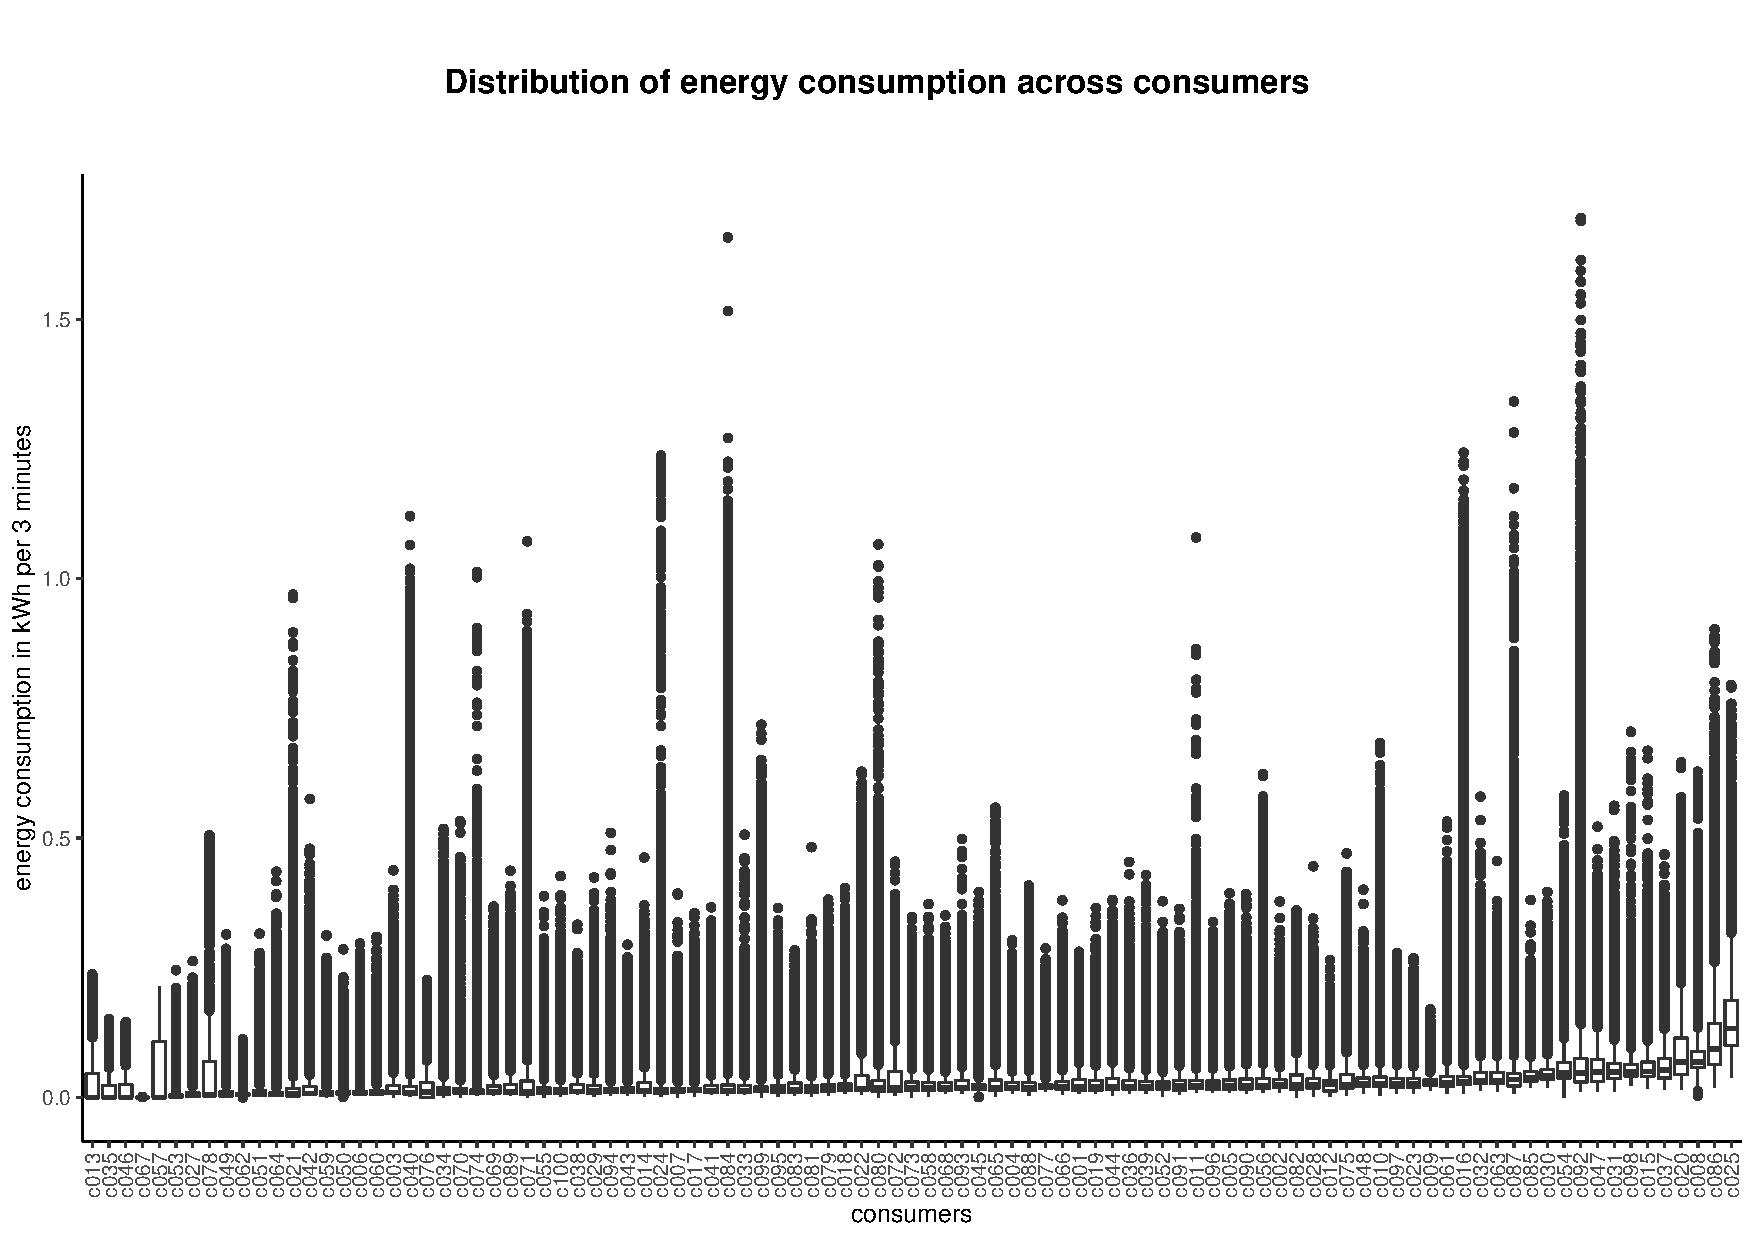
\includegraphics[width=\textwidth]{thesis/graphs/consumer_boxplots_consumption.jpg}
\caption[xxx]{xxx. \quantnet}
\label{Fig:boxplots_consumption}
\end{figure}

%%%%%%%%%%%
\subsubsection{Prosumer data sets}



%%%%%%%%%%%%%%%%%%%%%%%%%%%%%%%%%%%%%%%%%%%%%%%%%%%%%%%%%%%%%%%%%

\begin{itemize}

    \item Describe the data and its quality.
    \item How was the data sample selected?
    \item Provide descriptive statistics such as:
        \begin{itemize}
            \item time period,
            \item number of observations, data frequency,
            \item mean, median,
            \item min, max, standard deviation,
            \item skewness, kurtosis, Jarque--Bera statistic,
            \item time series plots, histogram.
        \end{itemize}
    \item For example:
        \begin{table}[ht]

        \begin{center}
            {\footnotesize
            \begin{tabular}{l|cccccccccc}
                \hline \hline
                           & 3m    & 6m    & 1yr   & 2yr   & 3yr   & 5yr   & 7yr   & 10yr  & 12yr  & 15yr   \\
                \hline
                    Mean   & 3.138 & 3.191 & 3.307 & 3.544 & 3.756 & 4.093 & 4.354 & 4.621 & 4.741 & 4.878  \\
                    StD    & 0.915 & 0.919 & 0.935 & 0.910 & 0.876 & 0.825 & 0.803 & 0.776 & 0.768 & 0.762  \\
                \hline \hline
            \end{tabular}}
        \end{center}
        \caption{Some descriptive statistics of location and dispersion for
        2100 observed swap rates for the period from February 15, 1999
        to March 2, 2007. Swap rates measured as 3.12 (instead of 0.0312). See Table
        \ref{Tab:DescripStatsRawDataDetail} in the appendix for
        more details.}
        \label{Tab:DescripStatsRawData}
        \end{table}

    \item Allows the reader to judge whether the sample is biased or to evaluate possible impacts of outliers, for
    example.

\end{itemize}


\newpage

\section{Results}\label{Sec:Results}

The results will be presented in two sections: First, the forecasting accuracy of the prediction models is evaluated and presented. Second, the results of the market simulation -- which is run once with the true consumption and production values and once with the predicted values -- are reported.


%%%%%%%%%%%%%%%%%%%%%%%%%%%%
%%%   Benchmark models   %%%
%%%%%%%%%%%%%%%%%%%%%%%%%%%%

\subsection{Evaluation of the prediction models}\label{Sec:Results;Subsec:Forecast}

Three prediction models where each applied to 82 consumer data sets and 12 prosumer data sets: the benchmark model (see Section~\ref{Sec:Method;Subsec:Benchmark}), the LSTM RNN model (see Section~\ref{Sec:Method;Subsec:LSTM}), and the LASSO model (see Section~\ref{Sec:Method;Subsec:LASSO}). All three prediction models are compared and evaluated using the error measures presented in Section~\ref{Sec:Method;Subsec:Error}.


%%%%%%%%%%%
\subsubsection{Consumption data}

The performance of the prediction values was tested on a quarter of the available data. That is, the prediction models were fitted on the consumption values from 01.01.2017 00:00 to 30.09.2017 00:00 which is equivalent to 131,040 data points per data set. For all 82 consumer data sets the models were fitted separately resulting in 82 distinct prediction models for each method. The fitted models were then used to make energy consumption predictions in 15-minute intervals on the data from 01.10.2017 00:00 to 01.01.2018 00:00. This equates to 8,836 predicted values per data set per model. The average performance of the three prediction models across all 82 data sets is shown in Table~\ref{Tab:avg_errormeasures}.
%
\begingroup\catcode`"=9
\begin{table}[ht]
{\footnotesize
    \csvreader[centered tabular=l|SSSSS,
    before reading=\sisetup{round-mode=places,round-precision=2,round-integer-to-decimal},
    filter not strcmp={\thecsvinputline}{1},
    table head=
    \hline\hline
     \multicolumn{1} {l}{\textbf{Model}} & \multicolumn{1} {|c}{\textbf{MAE}} & \multicolumn{1} {c}{\textbf{RMSE}} & \multicolumn{1} {c}{\textbf{MAPE}} & \multicolumn{1} {c}{\textbf{NRMSE}} & \multicolumn{1} {c}{\textbf{MASE}}\\
    \hline,
    no head,
    separator=comma,
    respect all,
    late after line=\\,
    table foot=\hline \hline]
    {thesis/tables/avg_errorMeasures.csv}{}%
    {\csvcolii & \csvcoliii & \csvcoliv & \csvcolv & \csvcolvi & \csvcolvii}}%
    \caption[Average error measures across all 82 consumer data sets]{Average error measures for the prediction of energy consumption across all 82 consumer data sets. \quantnet\href{ }{}}
    \label{Tab:avg_errormeasures}
\end{table}
\endgroup
%
As can be seen, LASSO and LSTM outperform the benchmark model according to MAE, RMSE, MAPE, and MASE by around 10 \%. Interestingly, due to the heavy penalty NRMSE puts on comparably large prediction errors, both sophisticated prediction methods perform worse according to NRMSE. A detailed analysis, however, reveals that this result is mainly driven, by extremely bad NRMSE scores of LSTM and LASSO on merely two of the 82 data sets. As can be seen in Figure~\ref{Fig:heatmapNRMSE}, the predictions on consumer data sets 027 and 076 have a particularly high NRMSE compared to all other data sets. However, this pattern is not present when use RMSE as error measure, as shown in Figure~\ref{Fig:heatmapRMSE}.
%
\begin{figure}[htbp]
 \centering
\includegraphics[width=\textwidth]{thesis/graphs/evaluation/c_heatmap_NRMSE.pdf}
\caption[Heatmap of NRMSE scores for consumption values]{Heatmap of  NRMSE scores for the prediction of consumption values per consumer data set. \quantnet\href{ }{}}
\label{Fig:heatmapNRMSE}
\end{figure}
%
\begin{figure}[htbp]
 \centering
\includegraphics[width=\textwidth]{thesis/graphs/evaluation/c_heatmap_RMSE.pdf}
\caption[Heatmap of RMSE scores for consumption values]{Heatmap of  RMSE scores for the prediction of consumption values per consumer data set. \quantnet\href{ }{}}
\label{Fig:heatmapRMSE}
\end{figure}
%

The LASSO model performs with a MAPE of 24.43 \% worse than in the implementation of \citet{Li:2017}, who achieved a score of 20.06 \%.
%
\begin{figure}
    \centering
    \includegraphics[width=.5\textwidth-0.15em]{thesis/graphs/evaluation/c_boxplot_MAE.pdf}
    \includegraphics[width=.5\textwidth-0.15em]{thesis/graphs/evaluation/c_boxplot_MAPE.pdf} \\
    
    \includegraphics[width=.5\textwidth-0.15em]{thesis/graphs/evaluation/c_boxplot_RMSE.pdf}
    \includegraphics[width=.5\textwidth-0.15em]{thesis/graphs/evaluation/c_boxplot_NRMSE.pdf} \\
    \caption{Caption}
    \label{fig:my_label}
\end{figure}


%%%%%%%%%%%
\subsubsection{Production data}




%%%%%%%%%%%%%%%%%%%%%%%%%%%%
%%%   Market simulation   %%%
%%%%%%%%%%%%%%%%%%%%%%%%%%%%

\subsection{Evaluation of the market simulation}\label{Sec:Results;Subsec:Simulation}



%%%%%%%%%%%
\subsubsection{True consumption and production values}



%%%%%%%%%%%
\subsubsection{Predicted consumption and production values}



%%%%%%%%%%%
\subsubsection{Cost due to prediction errors}



%%%%%%%%%%%%%%%%%%%%%%%%%%%%%%%%%%%%%%%%%%%%%%%%%%%%%%%%%%%%%%%%%

\begin{itemize}

    \item Organize material and present results.

    \item Use tables, figures (but prefer visual presentation):
        \begin{itemize}
            \item Tables and figures should supplement (and not duplicate) the
                text.

            \item Tables and figures should be provided with
            legends.\\
                {\it Figure~\ref{Fig:Resids} shows how to include and reference
                graphics. The graphic must be labelled before. Files must be in
                \texttt{.eps} format.}

                \begin{figure}[ht]
                \begin{center}
                    \includegraphics[scale=0.5,angle=0]{thesis/figures/graph.pdf}
                    \caption{Estimated residuals from model XXX. ...}
                    \label{Fig:Resids}
                \end{center}
                \end{figure}

            \item Tables and graphics may appear in the text or in
                the appendix, especially if there are many simulation results
                tabulated, but is also depends on the study and number of tables resp.
                figures. The key graphs and tables must appear in
                the text!
        \end{itemize}

    \item Latex is really good at rendering formulas:\\
        {\it Equation (\ref{Eq:SpecDens}) represents the ACs of a stationary
        stochastic process:
        \begin{equation}
            f_y(\lambda) = (2\pi)^{-1} \sum_{j=-\infty}^{\infty}
                           \gamma_j e^{-i\lambda j}
                         =(2\pi)^{-1}\left(\gamma_0 + 2 \sum_{j=1}^{\infty}
        \gamma_j \cos(\lambda j)\right)
                                        \label{Eq:SpecDens}
        \end{equation}
        where $i=\sqrt{-1}$ is the imaginary unit, $\lambda \in [-\pi,
        \pi]$ is the frequency and the $\gamma_j$ are the autocovariances
        of $y_t$.}

\newpage

    \item Discuss results:
        \begin{itemize}
            \item Do the results support or do they contradict economic theory ?
            \item What does the reader learn from the results?
            \item Try to give an intuition for your results.
            \item Provide robustness checks.
            \item Compare to previous research.
        \end{itemize}
\end{itemize}


\section{Conclusions}\label{Sec:Conc}



%%%%%%%%%%%%%%%%%%%
%%%   Summary   %%%
%%%%%%%%%%%%%%%%%%%%

\subsection{Summary of present research}\label{Sec:Conclusion;Subsec:Summary}



%%%%%%%%%%%%%%%%%%%%%%
%%%   Discussion   %%%
%%%%%%%%%%%%%%%%%%%%%%

\subsection{Discussion of results}\label{Sec:Conclusion;Subsec:Discussion}



%%%%%%%%%%%%%%%%%%%
%%%   Outlook   %%%
%%%%%%%%%%%%%%%%%%%

\subsection{Outlook and further research}\label{Sec:Conclusion;Subsec:Outlook}



%%%%%%%%%%%%%%%%%%%%%%%%%%%%%%%%%%%%%%%%%%%%%%%%%%%%%%%%%%%%%%%%%

\begin{itemize}

    \item Give a short summary of what has been done and what has been
    found.

    \item Expose results concisely.

    \item Draw conclusions about the problem studied. What are the
    implications of your findings?

    \item Point out some limitations of study (assist reader in judging validity
    of findings).

    \item Suggest issues for future research.

\end{itemize}




% ----------------
% --- appendix ---
% ----------------
\appendix

% literature
\newpage
\addcontentsline{toc}{section}{References}
\bibliography{thesis/99_literature.bib}

% figures
\newpage

\section{Figures}\label{App:Figures}

\subsection{Excluded consumer data sets}\label{App:Figures;Excluded}

\begin{figure}[ht]
    \begin{center}
        \includegraphics[]{thesis/grpahs/c021_cons.pdf}
        \includegraphics[]{thesis/grpahs/c046_cons.pdf}
        \includegraphics[]{thesis/grpahs/c053_cons.pdf}
        \includegraphics[]{thesis/grpahs/c057_cons.pdf}
        \includegraphics[]{thesis/grpahs/c078_cons.pdf}
        \includegraphics[]{thesis/grpahs/c080_cons.pdf}
        \caption[Consumer data sets excluded due to peculiarities in the consumption patterns]{Consumer data sets excluded due to peculiarities in the consumption patterns. \quantnet}
        \label{Fig:Resids2}
    \end{center}
\end{figure}


%%%%%%%%%%%%%%%%%%%%%%%%%%%%%%%%%%%%%%%%%%%%%%%%%%%%%%%%%%%%

\begin{figure}[ht]
    \begin{center}
        \includegraphics[scale=0.5,angle=0]{thesis/figures/graph.pdf}
        \caption{Estimated residuals (2) from model XXX. ...}
        \label{Fig:Resids2}
    \end{center}
\end{figure}


% tables
\newpage

\section*{Appendix B: Tables}\label{App:Tables}

\subsection*{B1 Summary statistics of total energy consumption and production} \label{App:Tables:totalcons}

\begin{table}[ht]
{\footnotesize
    \csvreader[centered tabular=l|......,
    filter not strcmp ={\thecsvinputline}{1},
    table head=
    \hline\hline
     & \multicolumn{1} {|c}{\textbf{Min}} & \multicolumn{1} {c}{\textbf{Q1}} & \multicolumn{1} {c}{\textbf{Median}} & \multicolumn{1} {c}{\textbf{Mean}} & \multicolumn{1} {c}{\textbf{Q3}} & \multicolumn{1} {c}{\textbf{Max}}\\
    \hline,
    no head,
    separator=comma,
    respect all,
    late after line=\\,
    table foot= \hline \hline]
    {thesis/tables/summarystats_total.csv}{}%
    {\csvcoli & \csvcolii & \csvcoliii & \csvcoliv & \csvcolv & \csvcolvi & \csvcolvii}}%
    \caption[Summary statistics of households' total consumption and production in 2017]{Summary statistics of households' total consumption and production in 2017. \quantnet}
    \label{App:Tab:cons_totalcons}
\end{table}



%%%%%%%%%%%%%%%%%%%%%%%%%%%%%%%%%%%%%%%%%%%%%%%%%%%%%%%%%%%%%%%%%%%%%%%%%%%%%%%%%%%%

% \begin{table}[ht]
%     \begin{center}
%         {\footnotesize
%         \begin{tabular}{l|cccccccccc}
%         \hline \hline
%                         & 3m    & 6m    & 1yr   & 2yr   & 3yr   & 5yr   & 7yr   & 10yr  & 12yr  & 15yr   \\
%             \hline
%                 Mean   & 3.138 & 3.191 & 3.307 & 3.544 & 3.756 & 4.093 & 4.354 & 4.621 & 4.741 & 4.878  \\
%                 Median & 3.013 & 3.109 & 3.228 & 3.490 & 3.680 & 3.906 & 4.117 & 4.420 & 4.575 & 4.759  \\
%                 Min    & 1.984 & 1.950 & 1.956 & 2.010 & 2.240 & 2.615 & 2.850 & 3.120 & 3.250 & 3.395  \\
%                 Max    & 5.211 & 5.274 & 5.415 & 5.583 & 5.698 & 5.805 & 5.900 & 6.031 & 6.150 & 6.295  \\
%                 StD    & 0.915 & 0.919 & 0.935 & 0.910 & 0.876 & 0.825 & 0.803 & 0.776 & 0.768 & 0.762  \\
%             \hline \hline
%         \end{tabular}}
%     \end{center}
%     \caption{Detailed descriptive statistics of location and dispersion for
%     2100 observed swap rates for the period from
%     February 15, 1999 to March 2, 2007. Swap rates measured as 3.12 (instead of 0.0312).}
%     \label{Tab:DescripStatsRawDataDetail}
% \end{table}


% code
\newpage

\section{Code}\label{App:Code}

\subsection*{Java REST API Client}\label{App:Code:API}

\inputminted[
firstline=
lastline=
]{java}{}


% --------------------------------------------
% --- last page: Declaration of Authorship ---
% --------------------------------------------

\newpage
\thispagestyle{empty}
%{\Large{\bf Declaration of Authorship}}\vspace{0.5cm}

\section*{Declaration of Authorship}

I, Michael Kostmann, hereby confirm that I have not previously submitted the present work for other examinations. I authored this Master's thesis independently and without use of others than the indicated sources. All passages which are literally or in general matter taken out of publications or other sources are marked as such. I understand that violations of these principles will result in proceedings regarding deception or attempted deception.
\\\vspace{0.5cm}

\noindent Berlin, November 12, 2018 \\\vspace{0.1cm}

\noindent Michael Kostmann



\end{document}
